\chapter{Methods for IACT Analyses}

\section{Coordinate Frames}
In the following the coordinate frames, that are used in this analysis,
are defined as per the ctapipe conventions \cite{karl_kosack_2019_3372211}.

\subsection{AltAz/Horizon Frame?}
A spherical coordinate system with the two angles azimuth and altitude.
This is used to describe the position of stars and shower origins.
In ctapipe, Azimuth is oriented east of north and altitude between the horizon 
and the zenith.

\subsection{CameraFrame}
A 2D cartesian frame to describe the shower in the focal plane.
The telescope orientation is defined as 
starting at the horizon, then pointed to the 
magnetic north in azimuth and up to zenith.
The two coordinates are defined as they are in CORSIKA:
$X$ points north and $y$ points west, with the telescope


\subsection{NominalFrame}
A common, spherical frame for all telescopes to perform 2D-reconstruction,
such as DISP-methods or intersection of Hillas-axes.
This is also necessary if telescopes are in divergent pointing mode.


% \subsection{GroundFrame}
% A cartesian frame with the origin in the array center. The positions of the
% telescopes is saved in the GroundFrame.

% \subsection{TiltedGroundFrame}
% For impact reconstruction, we dont need that?

\section{Monte Carlo Simulations}
Monte carlo simulations are a crucial part to 
understand the behaviour of an experiment. 
Simulating the underlying physic and the response of the experiment
allows the testing of new algorithms aswell as improving the general understanding
of the physical processes at work. 

For CTA, monte carlo simulations are done using a combination of the
programs CORSIKA and sim\_telarray.
While CORSIKA handels the formation and propagation of air showers,
the detector response can be simulated using the software
sim\_telarray \cite{BERNLOHR2008149}.

\subsection{Air Shower Simulation with CORSIKA}
CORSIKA \cite{heck1998corsika} is the standard software to simulate different types of
air showers in the field of astroparticle physics.
It allows to choose primary particles at will and
propagate them through the atmosphere, generating secondary particles, until
eventually the ground is reached.
Simulation options include, amongst other:
\begin{itemize}
  \item Amount of data to simulate
  \item Several random seeds
  \item Primary particle type
  \item Range and slope of the energy spectrum
  \item Alt/az range
  \item Models and parameters for the electromagnetic and hadronic interactions
  \item Models and parameters for the cherenkov light generation
  \item Atmospheric properties, such as the magnetic field
  \item Position and size of the detector grid
\end{itemize}

\subsection{Detector Simulation with sim\_telarray}
sim\_telarray is a software developed for the HEGRA IACT experiment,
but has since been developed to support arbitrary experiment setups \cite{BERNLOHR2008149}.
% It is able to simulate the full detector response and can be used to either
% perform complete simulations or use short-cuts in order to
% improve on the computational efficiency.

The main steps of the anaysis concern the optical raytracing of the cherenkov photons
and the simulation of the readout electronics and triggers.

The resulting data is meant to resemble the telescope raw data as closely as possible,
be it digitized pulse shapes or integrated signal sums.

\section{CTA's Processing Pipeline: ctapipe}
The main processing pipeline for low-level  CTA data is going to be ctapipe,
an open-source project hosted on github cite{ctapipe}.
It is currently in development and not all the planned 
features are yet available.
At the time of writing, the latest stable version is 0.7
\cite{karl_kosack_2019_3372211}.
Besides handling CTA-data, ctapipe also includes code to work with
other telescope geometries such as MAGIC.

\subsection{Telescope Level}
After recording an event, the data gets analyzed on telescope level.
This means that no information gets shared between telescopes.
The initial step consists of calling the
CameraCalibrator class. This includes an optional
data volume reduction (?) and an integration of the recorded waveforms.
In this step the information gets reduced to two values per pixel:
Charge and pulse time.

The resulting 2D-images gets cleaned to select the signal pixels,
that get used for further analysis.
An illustration of the cleaning step 
for a simulated shower in the LSTCam is given in figure \ref{fig:shower_cleaning}.
The default tailcuts cleaning algorithm works with two thresholds on the 
pixel charge. All pixels above the upper threshold with a set amount of neighbouring 
pixels above that threshold get selected, aswell as 
all pixels above the lower threshold with the same set amount of neighbouring pixels
above the upper threshold.
During the course of this thesis, I added a second algorithm, that is used by the FACT-collaboration 
and additionaly makes use of the pulse time information.
It works in a similar way, but with additional steps removing pixels, that arrived
at distant times.

\begin{figure}
	\centering
	\captionsetup{width=0.9\linewidth}
	\begin{subfigure}{.42\textwidth}
  		\centering
  		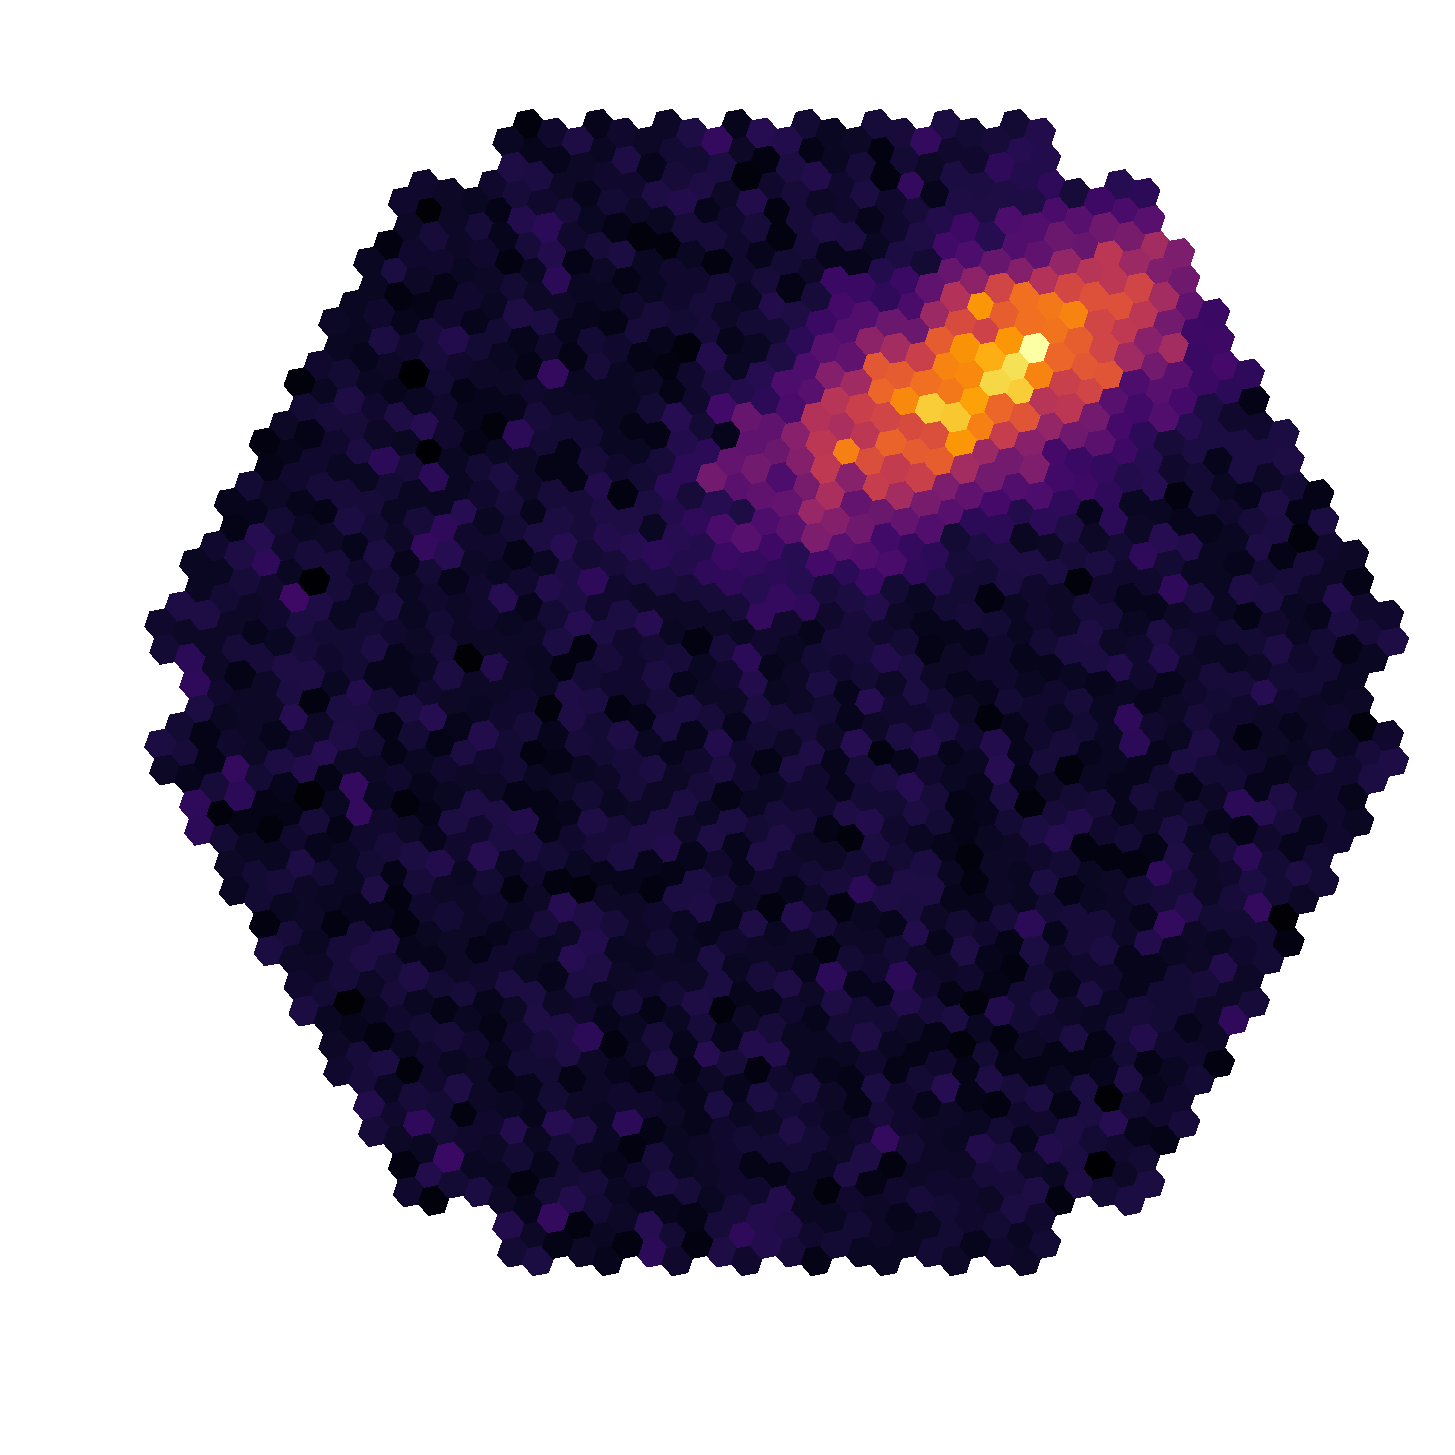
\includegraphics[width=\linewidth]{Plots/hillas_raw.pdf}
	\end{subfigure}%
	\begin{subfigure}{.48\textwidth}
 		\centering
		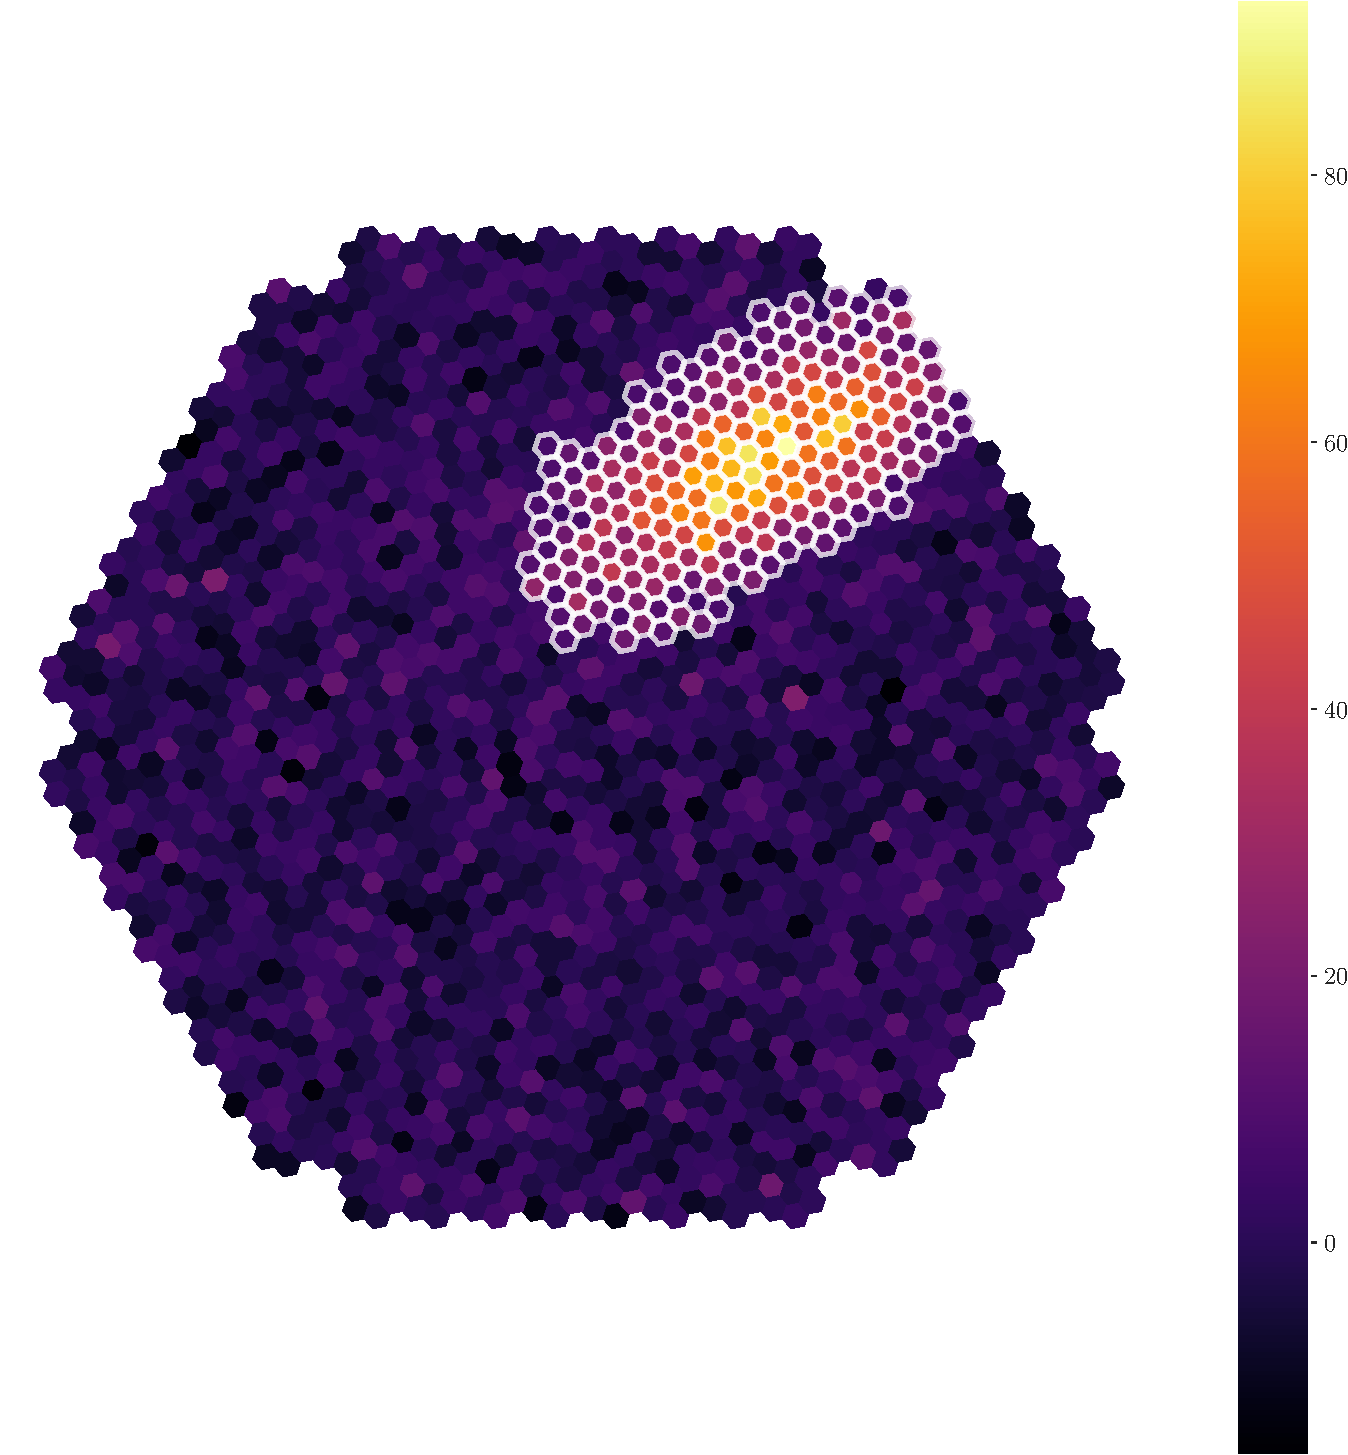
\includegraphics[width=\linewidth]{Plots/hillas_cleaned.pdf}
	\end{subfigure}
	\caption{
		Left: The signal directly after
		the waveform integration. The non-signal pixels contain a lot of noise. \\
		Right: Image after the cleaning-algorithm has been 
		applied. The highlighted pixels are used for further analysis steps.}
	\label{fig:shower_cleaning}
\end{figure}

Several parameters can be calculated on the charge values, the most prominent ones are the 
hillas parameters, illustrated in figure \ref{fig:hillas_params}.

\begin{figure}
	\centering	
	\captionsetup{width=0.9\linewidth}
	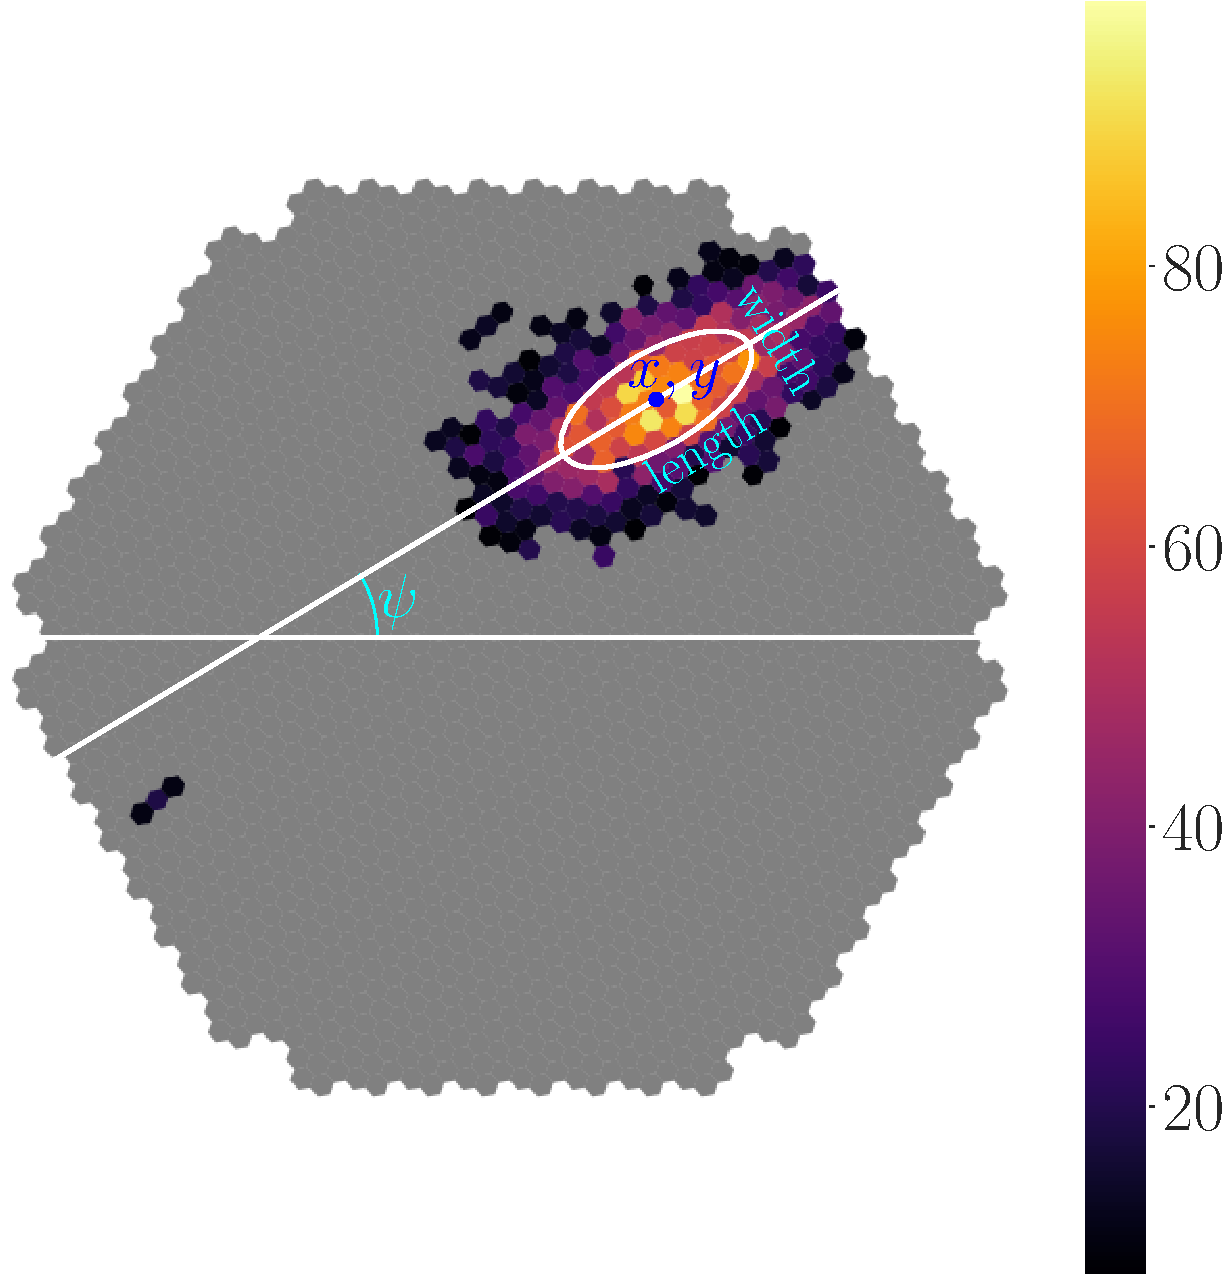
\includegraphics[width=.6\textwidth]{Plots/hillas_cleaned_params.pdf}
	\caption{The same cleaned shower-image as in figure \ref{fig:shower_cleaning}
	with the hillas-parameters calculated and marked in the camera frame.
	The parameters $\phi$, $\psi$, $x$ and $y$ describe the 
	orientation and position of the shower ellipse in the camera frame.
  The blue line marks the main shower axis.}
	\label{fig:hillas_params}
\end{figure}

Other parameters include variations of the leakage and concentration of the shower image.
Leakage describes how much of the signal is located in the outermost pixels of the camera, 
concentration describes how contained the image is by comparing the light in 
few selected pixels with the sum of all pixels.

In addition, I added an algorithm, that counts the seperated clusters in the image,
the sum of which is referred to as number of islands.

A class of parameters, that is evaluated on the pulse times, are the timing
parameters. These describe the temporal evolution of the image by fitting
a 1D-polynom on the pulse times. The parameters of the fit and the deviation
between observed and estimated pulse times are saved as the timing parameters. 


\subsection{Array Level}
From the image descriptions, high level features can be calculated.
These include the primary particle type and energy aswell as 
the shower origin and impact point.

Since CTA is going to be a stereoscopic experiment,
the information of multiple telescopes can be combined to
reconstruct propoerties of the shower and its primary particle.

An algorithm, that makes use of the stereoscopic array planned for CTA,
is the HillasReconstructor, which works based on the hillas parametrisation
of the images.

For each triggered telescope, a 2D-plane is drawn into the spatial 3D-space based on the main shower 
axis and the telescope orientation. These planes intersect and 
the weighted average of all intersections yields the 
main interaction point of the observed shower and the source position.
Intersecting the main shower axes on the ground frame leads to 
an estimation of the impact point of the shower (IS THAT HOW IT WORKS?).
For a general illustration see figure \ref{fig:hillas_reconstructor}.

Right now this is the default reconstruction algorithm inside ctapipe.
The current implementation does not provide an 
estimation for the uncertainty of the reconstructed parameters.

\begin{figure}
	\centering
	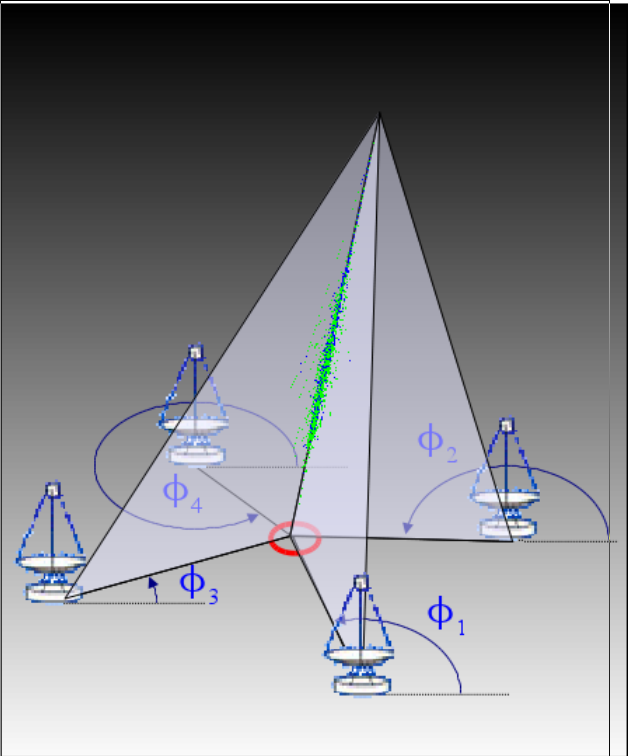
\includegraphics[width=0.6\textwidth]{images/hillas_reco.png}
	\caption{Illustration of a stereoscopic reconstruction of the source position.
    From each telescope a plane is drawn, the direct intersection 
    on the ground leads to the impact point (red circle).
    The image is taken from a habilitation thesis by 
    Mathieu de Naurois \cite{hillas_reco}.
    Not included is the reconstruction of the main interaction point
    and source position, which would be obtained by averaging the plane
    intersections.}
	\label{fig:hillas_reconstructor}
\end{figure}

Since this method inherently requires a stereoscopic experiment
and multiple triggered telescopes, it will not work for a single telescope.


% HillasIntersection auch noch erklären als Motivation für DISP?
% Aber dann müsste man eigentlic dagegen benchmarken...


\section{Additional Approaches}
With all the image features calculated and lots of monte carlo
data available, machine learning algorithms can perform
very well in these kind of analyses.
Two use cases involve the DISP-method
and the gamma-/hadron-separation.

\subsection{The DISP-Method}
For the reconstruction of the source position
one possible way involves using the DISP-method in some way.
Its advantage over the HillasReconstructor lies in the ability to
perform purely monoscopic reconstructions.

As basic estimation one can predict the shower origin by 
transforming the center of gravity (cog) of the image onto the sky plane.
The DISP-method assumes that the 
center of gravity is displaced relative to the
real source position depending on the angle the photon arrived at the telescope.
If one assumes the true source position to be on the main shower axis of the ellipse,
finding this position simplifies to finding a single point on the main shower axis, that 
can then be transformed to the horizon frame.
The calculation of the DISP is based on either lookup tables or machine learning,
both based on the use of monte carlo data.

Monoscopic experiments, that make use of the DISP method, need to resolve the head-tail-ambiguity:
The DISP calculation itself only grants the distance between
cog and source position, leaving two valid points.
One way to solve this problem is to treat it as classification task with two
classes $\pm1$, denoting the two directions to move from the cog.
Similar models as for the DISP can then be calculated using monte carlo data.

Stereoscopic experiments can resolve this ambiguity by combining the images from 
multiple telescopes, as can be seen in figure \ref{fig:stereo_shower}.

\begin{figure}
	\centering
	\captionsetup{width=0.9\linewidth}
	\hspace*{0.1\textwidth}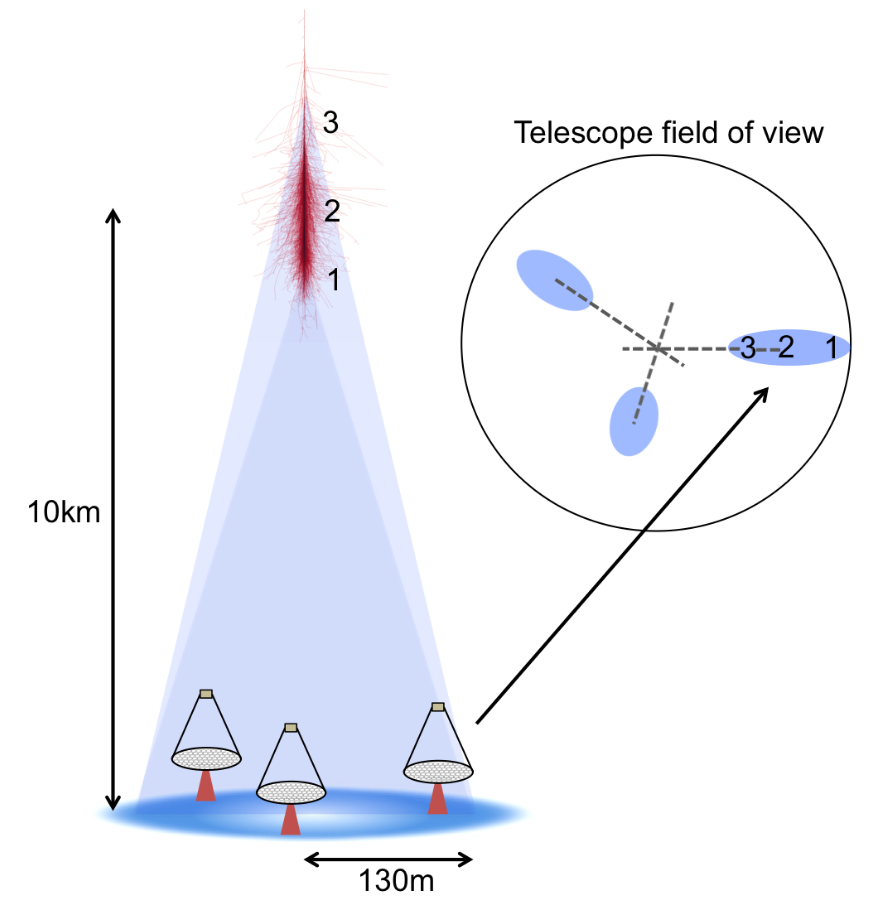
\includegraphics[width=0.9\textwidth]{images/stereo_shower.png}
	\caption{An illustration of an air shower captured with multiple telescopes.
		Each telescope captures an elliptic image.
		The image axes get intersected to reconstruct the arrival direction
		of the primary particle.
	    The image is taken from \cite{2015arXiv151005675H}.}
	\label{fig:stereo_shower}
\end{figure}

\subsection{Classification}
One important task, that ctapipe does not handle (yet?), is the classification of
the primary particle. If looking at a gamma source this simplifies
to binary classification with the two classes signal/gamma and background/hadron.

This can be done on telescope or array level, using all the features from the previous
steps. Models are trained on the monte carlo data.

\subsection{Machine Learning}
The mentioned approaches rely on the training of machine learning models on
monte carlo data.
With full information available on the simulated data, supervised
algorithms such as random forests become feasible.

Methods based on Decision Trees work by recursively partitioning
the parameter space until the remaining samples behave similar enough.
Tree-based methods can be applied to both classification and regression tasks.

Forest methods combine multiple tree predictors to get more stable
predictions.

\subsubsection{Supervised learning}
In the task of supervised machine learning a model is trained on a
dataset with full information available.
Training in this context means to optimize the parameters of a 
model to get a better prediction on the training data.
This data will come from Monte Carlo simulations in our case, but
could also be e.g. historical or hand labeled datasets in other contexts.
The trained model can then later be used to estimate features on a dataset, which
lacks the needed information.

We define a dataset as having a number of samples with a fixed number of
features each. In the following we split
the features of our dataset into a set of input variables $X$ and
a set of output variables $y$.

The naming convention for
these sets follows the one of scikit-learn
\cite{scikit-learn}, \cite{sklearn_api}, a python package for
machine learning algorithm, that will be used for the
machine learning models in this analysis.
Other terminologies for the two feature sets include
predictors or independent variables for the input, and
responses or dependent variables for the output.

\subsubsection{Classification}
In (supervised) classification tasks, the task is to predict of which of some
predefined classes the given sample is a member. The possible solutions for $y$
are from a discrete set of values in
contrast to a regression problem with a continuous solution space.
A model that performs classification on data is referred to as a
classifier.

The simplest and most popular case of classification problems
is \textit{binary classification} \cite{sokolova2009systematic}.
In this case only two distinct
classes exist, which fortunately is all thats needed for
the basic background rejection used later.
% A common example for a classification problem is an Email spam filter,
% where mails get categorized in at least two categories based
% on their content and meta data \cite{DBLP:journals/corr/cs-CL-0006013}.

For binary classification a set of measures
to define the quality of the prediction can be defined, starting with the confusion matrix
shown in table \ref{tab:confusion},
with $pos$ referring to the true label of the positive (i.e. signal)
and $neg$ referring to the label of the negative (i.e. background) class.

\begin{table}
    \caption{Definition of the confusion matrix for binary classification.
    The main diagonal includes the correct predictions, wrong predictions are on the off diagonal.}
    \begin{center}
        \begin{tabular}{ l| l l}
            %\hline
            {} & Predicted as $pos$ & Predicted as $neg$ \\
            \hline
            $pos$ & true positive ($tp$) & false negative ($fn$) \\
            %\hline
            $neg$ & false positive ($fp$) & true negative ($tn$) \\
            %\hline
        \end{tabular}
    \end{center}
    \label{tab:confusion}
\end{table}

An ideal classification would result in
\begin{equation*}
  fp = fn = 0.
\end{equation*}

As this can usually not be achievd, different measures
can be used to examine the classifiers performance
depending on the goal of the analysis.
Some of the more common ones are listed in table \ref{tab:class_metrics}.
(Nur die genutzten? Oder die erwähnen?)

\begin{table}
    \caption{Popular metrics for binary classification tasks.}
    \begin{center}
        %\caption{
         % Common metrics for classification tasks, taken from \cite{sokolova2009systematic}.}
        \begin{tabularx}{\textwidth}{l c X}
            %\hline
            Measure & Formula & Interpretation \\
            \hline
            Accuracy & $\frac{tp+tn}{tp+fn+fp+tn}$ & Class agreement on both labels \\
            Balanced Accuracy & $\frac{1}{2}(\frac{tp}{tp+fn}+\frac{tn}{fp+tn})$ & Classifier’s ability to avoid false classification \\
            Precision & $\frac{tp}{tp+fp}$ & Class agreement with the positive labels given by the classifier \\
            Recall/Sensitivity & $\frac{tp}{tp+fn}$ & Effectiveness of a classifier to identify positive labels \\
            F$_{\beta}$-score & $\frac{(\beta^2+1)tp}{(\beta^2+1)tp+\beta^2fn+fp}$ & Harmonic mean between precision and recall with choosable $\beta$ \\
            Specificity & $\frac{tn}{fp+tn}$ & How effectively a classifier identifies negative labels \\
        \end{tabularx}
    \end{center}
    \label{tab:class_metrics}
\end{table}

A classifier can also be used to predict a class probability.
For the case of binary classification, this can be a number between 0 and 1,
with 0 being one class and 1 being the second.
The classifier threshold is then the value at which the separation into the two classes happens.
One can then calculate the Area Under the Curve (AUC) with regard to the Receiver Operating Characteristic (ROC) curve.
The ROC-curve is gained by plotting the true positive rate against the false positive rate while varying the classifier threshold.
The area under the (normalised) ROC-curve is thus a measure for whether the classifier will
rank a randomly chosen positive sample higher than a randomly chosen negative sample \cite{FAWCETT2006861}.

\subsubsection{Regression}
Regression is the task of predicting a continuous variable
from a set of input variables.
The simplest approach
to this problem is the ordinary linear least squares method.

Given an unrestricted linear model
\begin{align}
	y &= X\beta + e \\
	E(y) &= X\beta \\
	Cov(y) &= \sigma^2 I_n
\end{align}
with a measured vector $y$, the design matrix $X$,
an unknown parameter vector $\beta$, a random error $e$
and pairwise orthogonal features $y_i$,
the least-squares solution is given by the solution of
the minimizing problem in equation \ref{eq:min_least_squares}.

\begin{equation}
	\min_{\beta\in\mathbb{R}^k} \lVert y - X\beta \rVert
	\label{eq:min_least_squares}
\end{equation}

If $(X^TX)^{-1}$ exists, the unique solution for the
least square estimation of $\beta$ becomes:
\begin{equation}
	\hat{\beta} = X^+ y,
\end{equation}

with the Moore-Penrose inverse $X^+ = (X^TX)^{-1}X^T$.
The estimation of $y$ is then:
\begin{equation}
  \hat{y} = X\hat{\beta}.
\end{equation}

The metric, that is minimized by the least-squares solution
is the Mean Squared Error (MSE).

Other metrics for regression tasks include the
Root-Mean-Squared-Error(RMSE),
Mean-Absolute-Error(MAE)
or the Coefficient of Determination ($R^2$), all of which are listed in table
\ref{tab:regr_metrics}.

\begin{table}
  \caption{Popular metrics for a regression problem with $n$ samples.}
  \begin{center}
    \begin{tabularx}{\textwidth}{l c X}
      Measure & Formula & Interpretation \\
      \hline
      Mean squared error & $\frac{1}{n}\sum_i^n |y_i-\hat{y_i}|$ & Prediction error disregarding the direction of over- and underprediction \\
      Mean absolute error & $\frac{1}{n}\sum_i^n (y_i-\hat{y_i})^2$ & For an unbiased predictor: Variance of the regressor. Heavily weights outliers. \\
      Coefficent of Determination & $1 - \frac{\sum_i^n (\bar{y_i}-\bar{y})^2}{\sum_i^n (y_i-\bar{y})^2}$ & Share of observed variance that is explained by the model.\\
    \end{tabularx}
  \end{center}
  \label{tab:regr_metrics}
\end{table}

Many metrics closely connected to these metrics exist, such as the root mean squared error (RMSE)
or the mean absolute percentage error (MAPE).

\subsubsection{Decision Trees and Random Forests}
A simple (binary) decision tree
for an example dataset with 50 proton and 50 gamma
events is shown in figure \ref{fig:03_tree}.

\begin{figure}
  \centering
  \captionsetup{width=0.9\linewidth}
  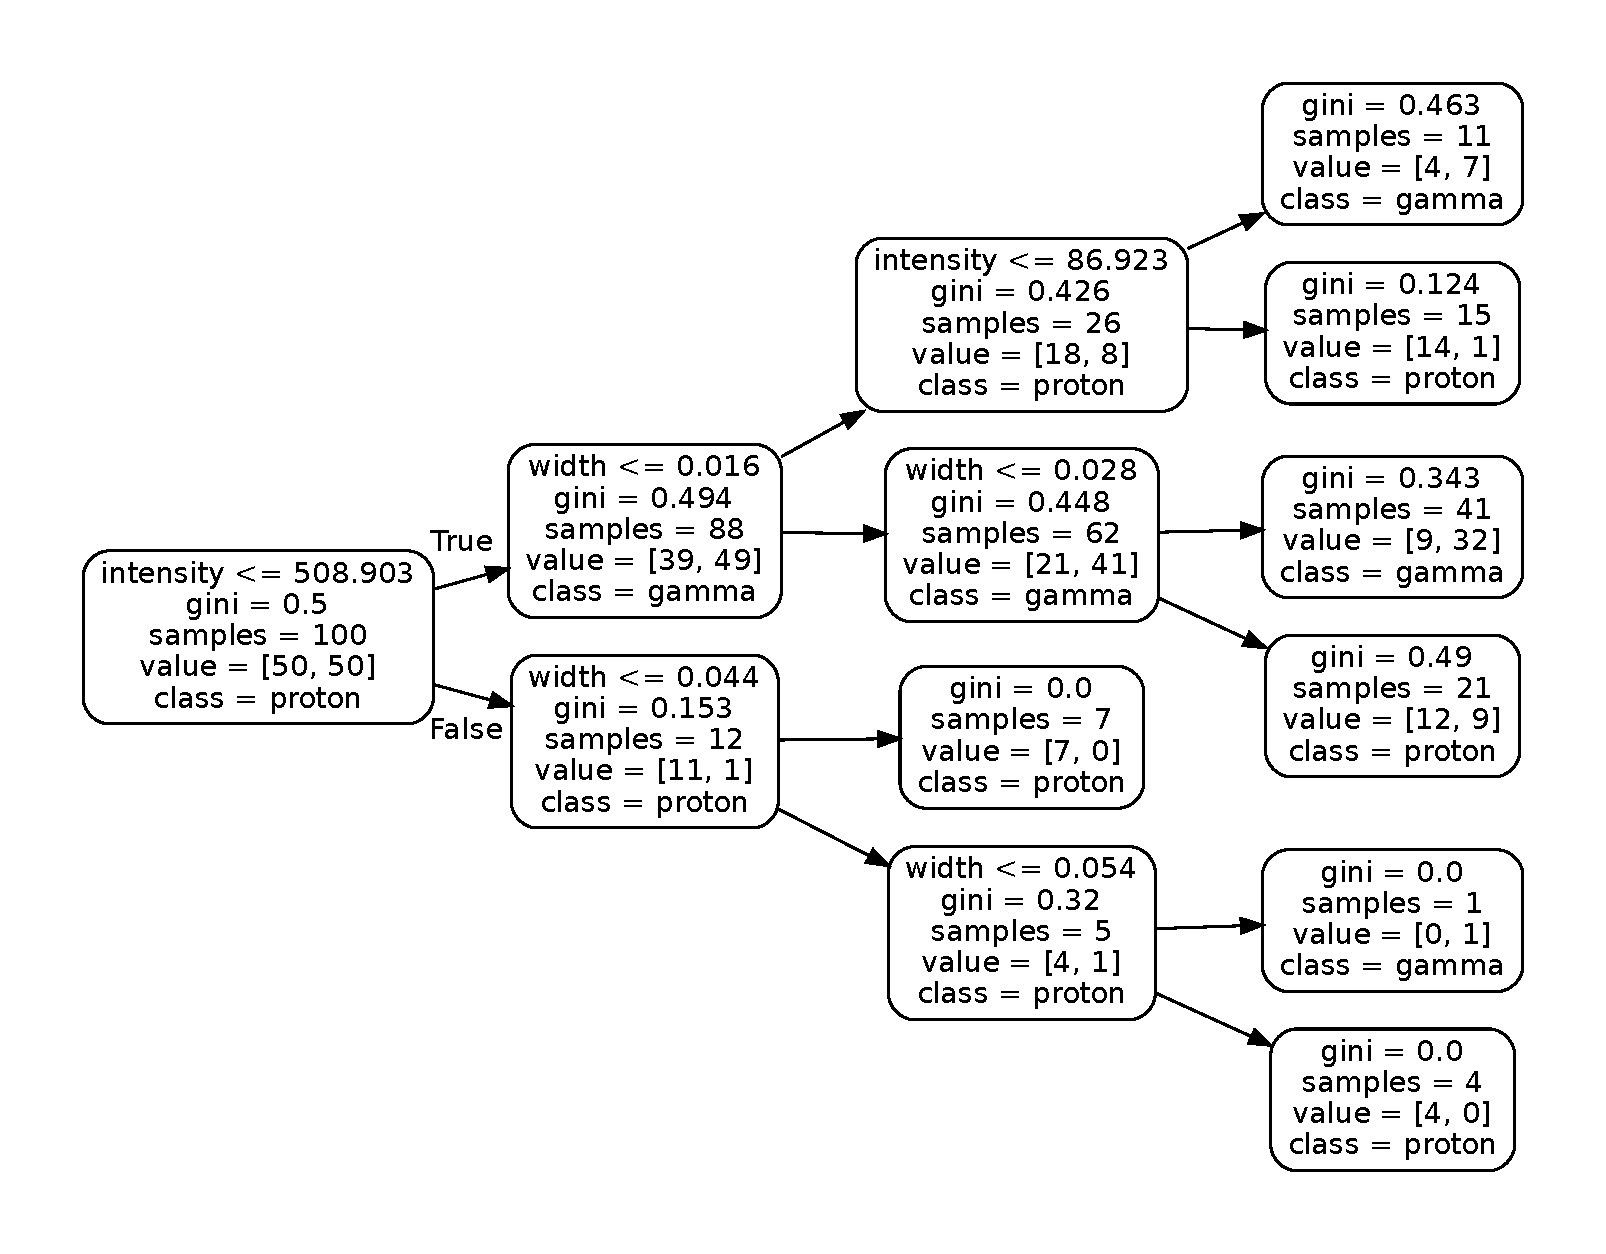
\includegraphics[width=0.9\textwidth]{Plots/decision_tree.pdf}
  \caption{A decision tree for a small sample dataset consisting of 50 proton and
  50 gamma events. The tree is capped at a depth of 4 and splits only on the 
  features width, length and intensity. On the training data, this tree reaches an
  accuracy of \num{0.81}.}
  \label{fig:03_tree}
\end{figure}

Starting from the root node, a binary split is performed to
split up the data. For each resulting node, additional splits are performed
until a stopping criterion is reached.
Choosing the optimal split is defined as minimizing a
pre-defined measure.

For classification tasks this means reducing the class impurity in the node.
Often used measures
to quantify the impurity are gini coefficient or the
cross-entropy \cite{hastie2017springer}.
Both are defined in equation \ref{eq:gini_ce}

\begin{align}
	\text{Gini impurity: } &= \sum_{k=1}^K \hat{p}_{mk}(1-\hat{p}_{mk}) \\
	\text{Cross-entropy: } &= -\sum_{k=1}^K \hat{p}_{mk}\log{\hat{p}_{mk}},
  \label{eq:gini_ce}
\end{align}

with $p_{mk}$ denoting the proportion of class $k$ in node $m$.

A stopping criterion can be defined as the measure reaching a
a defined threshold or not improving anymore.
Alternatively the tree can stop at a predefined depth to
avoid overly complex models.

For regression tasks scikit-learn uses the mean squared error
or mean absolute error and the same principles apply.

The implementation in sklearn is based on the one by
Leo Breiman et al \cite{breimanclassification}.
A single tree performs binary splits $\Theta = (j, t_m)$
at each node $m$ in order to split
the data at this node $Q$ into two subsets
$Q_\text{left}$
and
$Q_\text{right}$.
The split consists of a feature $j$ and a threshold $t_m$ and is
chosen in a way to minimize the given measure.
Features, that are more important for the task, will
thus appear at the top nodes of the tree.


While decision trees have the benefit of providing
easily interpretable, low bias models there are some drawbacks to this
approach, namely \cite{hastie2017springer}:
\begin{itemize}
  \item{Instability, high variance}
  \item{Lack of Smoothness}
  \item{Difficulty in Capturing Additive Structure}.
\end{itemize}

One approach to reduce these problems is the construction of
random forests \cite{Breiman2001}.

The main idea behind random forests is to use multiple
decision trees to suppress the problems single trees have, while
keeping their advantages.
For this to work, the individual trees should  be correlated.
Consequently the trees cannot all be constructed the same way.
To make sure the individual trees
- and their predictions -
are somewhat independent from each other,
randomness has to be introduced to the construction of the tree.
In random forests this is on the one hand achieved by giving each tree a
random subsample from the training data, obtained with bootstrapping \cite{efron1992bootstrap}.
Another source of randomness is to perform splits on a node
based on only a random subsample of the available features.

The prediction of the random forest in scikit learn is then the average of
the single trees predictions.
In the case of a classification task, the probabilistic predictions for each class
get averaged.
